\documentclass[tikz, border=10pt]{standalone}
\usepackage{tikz}
\usetikzlibrary{shapes.geometric, arrows.meta, positioning}

\begin{document}

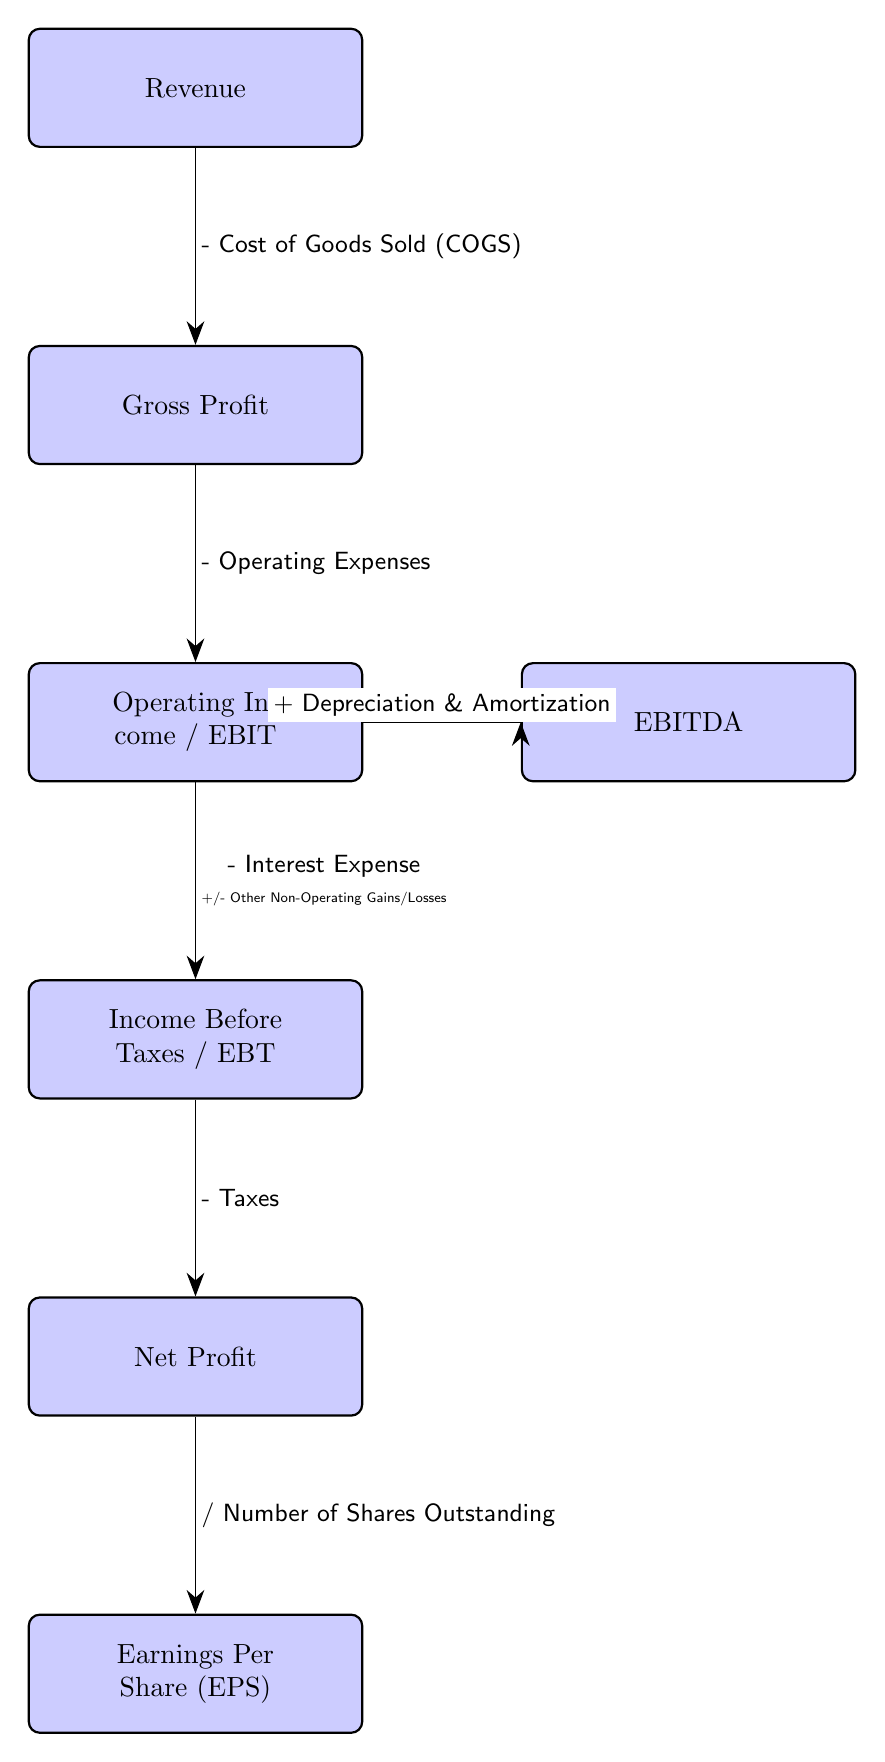
\begin{tikzpicture}[
    % Set distances between nodes
    node distance=2.5cm and 2cm,
    % Style for the main boxes (nodes)
    box/.style={
        rectangle,
        rounded corners,
        draw=black,
        thick,
        fill=blue!20,
        text width=4cm,
        align=center,
        minimum height=1.5cm
    },
    % Style for the labels on the connections (edges)
    edge_label/.style={
        midway,
        fill=white,
        inner sep=2pt,
        font=\small\sffamily
    }
]

% 1. Place the nodes using relative positioning
\node[box] (revenue) {Revenue};
\node[box, below=of revenue] (gross_profit) {Gross Profit};
\node[box, below=of gross_profit] (op_income) {Operating Income / EBIT};
\node[box, below=of op_income] (ebt) {Income Before Taxes / EBT};
\node[box, right=of op_income, node distance=5cm] (ebitda) {EBITDA};
\node[box, below=of ebt] (net_profit) {Net Profit};
\node[box, below=of net_profit] (eps) {Earnings Per Share (EPS)};

% 2. Draw the arrows (edges) and place the labels
\draw[-{Stealth[length=3mm]}] (revenue) -- (gross_profit)
    node[edge_label, right] {- Cost of Goods Sold (COGS)};

\draw[-{Stealth[length=3mm]}] (gross_profit) -- (op_income)
    node[edge_label, right] {- Operating Expenses};

\draw[-{Stealth[length=3mm]}] (op_income) -- (ebt)
    node[edge_label, right, align=center] {- Interest Expense \\ \tiny{+/- Other Non-Operating Gains/Losses}};

% This is the branch off to the right for the EBITDA calculation (FIXED LINE)
\draw[-{Stealth[length=3mm]}] (op_income.east) -| (ebitda.west)
    node[edge_label, above, pos=0.25] {+ Depreciation \& Amortization};

\draw[-{Stealth[length=3mm]}] (ebt) -- (net_profit)
    node[edge_label, right] {- Taxes};

\draw[-{Stealth[length=3mm]}] (net_profit) -- (eps)
    node[edge_label, right] {/ Number of Shares Outstanding};

\end{tikzpicture}

\end{document}